\documentclass{article}
\usepackage[a4paper, tmargin=1in, bmargin=1in]{geometry}
\usepackage[utf8]{inputenc}
\usepackage{graphicx}
\usepackage[justification=centering]{caption}

% \usepackage{parskip}
\usepackage{pdflscape}
\usepackage{listings}
\usepackage{hyperref}
\usepackage{caption}
\usepackage{subcaption}
\usepackage{float}
\usepackage{amsmath}
\DeclareMathOperator*{\argmax}{\arg\!\max}
\title{CS 747 : Foundations of Intelligent Learning Agents Assignment 3}
\author{Arka Sadhu - 140070011}
\date{\today}

\begin{document}
\maketitle

\section{Q-learning}
For q-learning the following has been done:
\begin{itemize}
\item We continue a particular episode until a terminal state is reached, or the number of iterations for the particular episode has crossed a certain threshold, in this case 1000.
\item When the agent is initialized, a q-table for each corresponding state and action is initialized. Here we initialize it with all 0's. A learning rate is suitably chosen.
\item The first action is given as random. The reward, next state and event is received from the server. If the goal is reached, the reward is 100, anything else is awarded a reward of -1. The event is either continue, terminated or goal reached.
\item We note the events. If it is either terminated or goal reached we update the corresponding q-table and then start a new episode. If it is continued we only udpate the q-table.
\item The update of q-table includes two steps. First the action which gives the highest q-value in the next state is chosen. This is then used to update the value in the q-table corresponding to current state and current action.
  $$Q[s, a] = Q[s, a] + \alpha * (reward +  \gamma * \max_a Q(s', a) - Q(s, a))$$
\item When asked for the next action, the agent chooses the action in an epsilon greedy manner from the q-table values corresponding to the current state. The epsilon is decayed in $\frac{1}{n}$ manner where n is the episode number.
\item For plotting the graphs, we have used 50 random seeds for each instance 0 and 1, and then taken the average reward for each episode.
\end{itemize}

\begin{figure}[H]
  \centering
  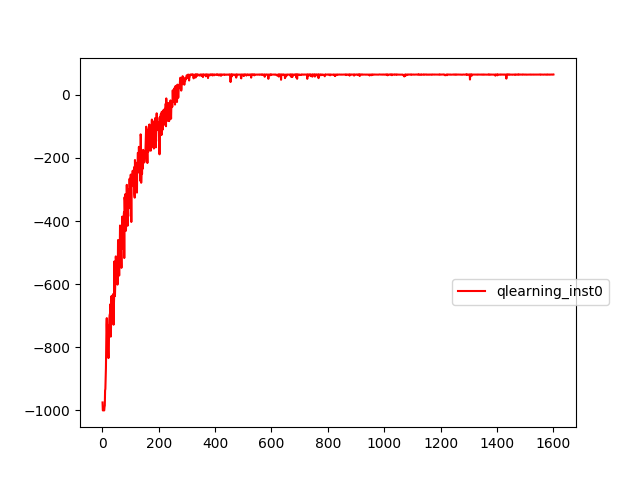
\includegraphics[scale=0.5]{images/qlearn_instance_0}
  \caption{Q-learning for instance 0}
  \label{fig:ql0}
\end{figure}

\begin{figure}[H]
  \centering
  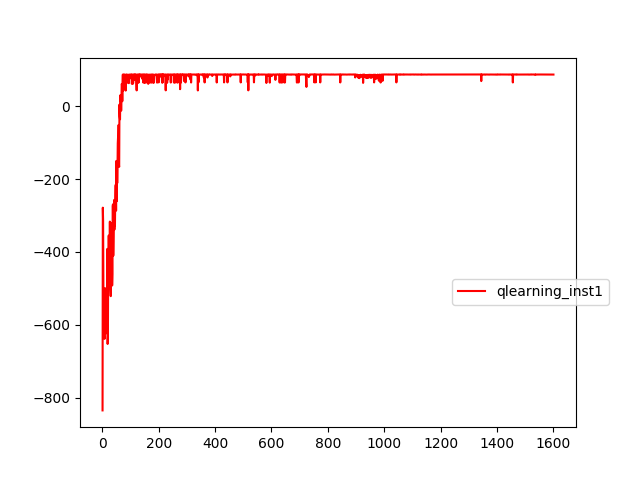
\includegraphics[scale=0.5]{images/qlearn_instance_1}
  \caption{Q-learning for instance 1}
  \label{fig:ql1}
\end{figure}

\begin{figure}[H]
  \centering
  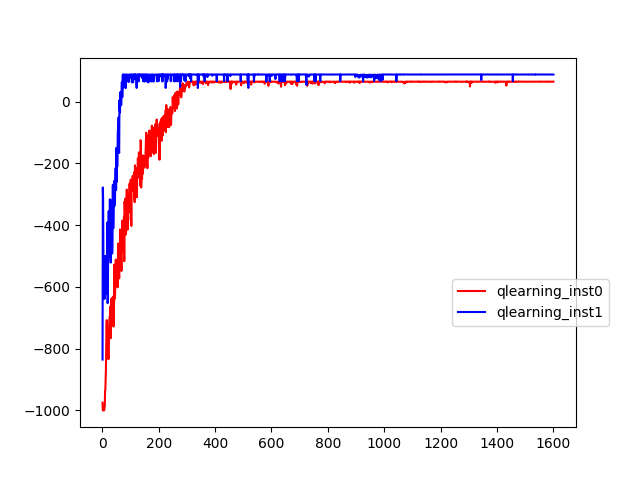
\includegraphics[scale=0.5]{images/qlearn_instance_0_1}
  \caption{Q-learning both instance 0 and 1}
  \label{fig:ql01}
\end{figure}
\section{Sarsa ($\lambda$)}
For sarsa ($\lambda$) the following has been done:
\begin{itemize}
\item All the initializations are the same as in Q-learning. The only difference is that we initialize a new matrix called the eligibility matrix of the same size of the q-table to all zeros. Also we choose the first action at random.
\item The same steps are followed as in Q-learning when the reward, next state and the event is given. As an extra we re-initialize the eligibility trace to all zeros when the episode either terminates or goal is reached. Next we update the q-table and the eligibility trace.
\item Now given the new state, we choose a new action using some epsilon greedy method on the q-table. Here this strategy is kept the same as that followed for q-table. We call this action as a'.
\item We use this a' for computing the update. First we initialize another variable $\delta$ which is computed as :
  $$\delta = reward + \gamma * Q(s', a') - Q(s, a)$$
\item Next depending on the trace strategy we update the eligibility trace corresponding to the current state and action. If accumulative trace is used then we add 1 to the existing value. If replacing trace is used we re-assign the existing value to 1.
\item Then for all states and all actions (basically the whole matrix) we do the following udpates:
  $$Q = Q + \alpha * \delta * eligibility\_trace$$
  $$eligibility\_trace = \gamma * \lambda * eligibility\_trace$$
\item For the next action we choose a'.
\item Again for the plots we have averaged over 50 random seeds for each episode.
\end{itemize}

\begin{figure}[H]
  \centering
  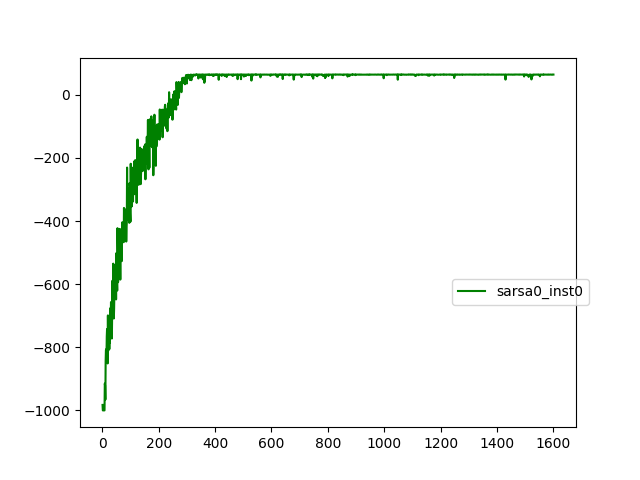
\includegraphics[scale=0.5]{images/sarsa0_instance0}
  \caption{Sarsa 0 for instance 0}
  \label{fig:s0i0}
\end{figure}
\begin{figure}[H]
  \centering
  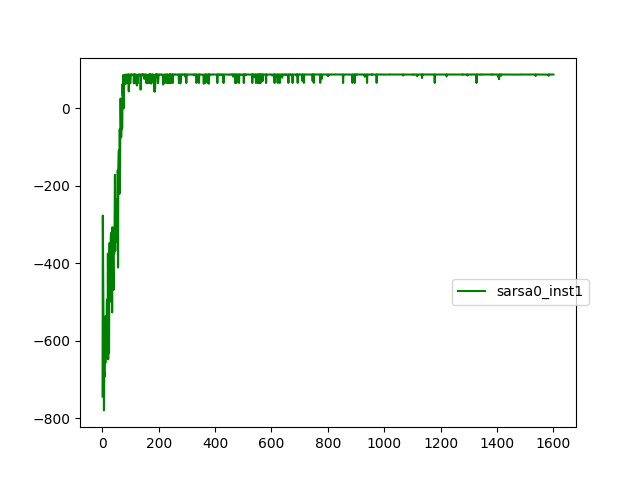
\includegraphics[scale=0.5]{images/sarsa0_instance_1}
  \caption{Sarsa 0 for instance 1}
  \label{fig:s0i1}
\end{figure}
\begin{figure}[H]
  \centering
  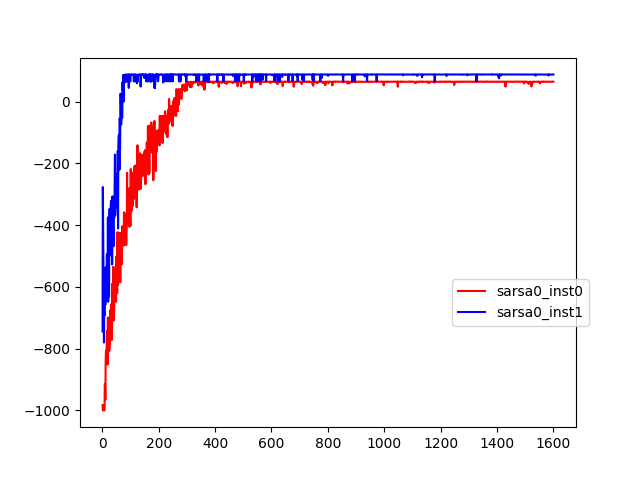
\includegraphics[scale=0.5]{images/sarsa0_instance_0_1}
  \caption{Sarsa 0 for instance 0, 1}
  \label{fig:s0i01}
\end{figure}

\begin{figure}[H]
  \centering
  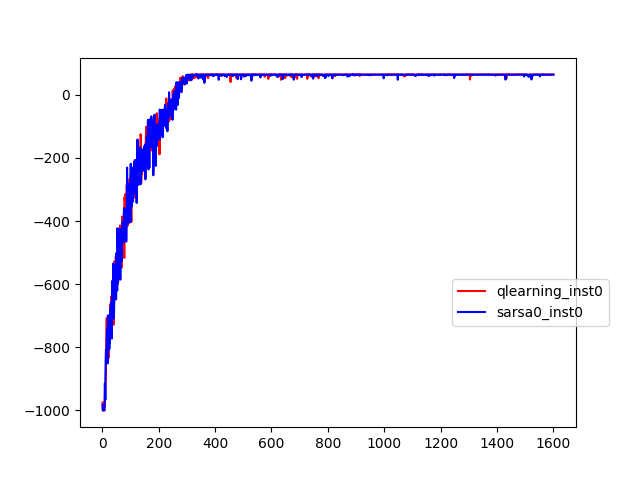
\includegraphics[scale=0.5]{images/qlearn_sarsa0_instance0}
  \caption{Q-learn and Sarsa0 for instance 0}
  \label{fig:ins0}
\end{figure}

\begin{figure}[H]
  \centering
  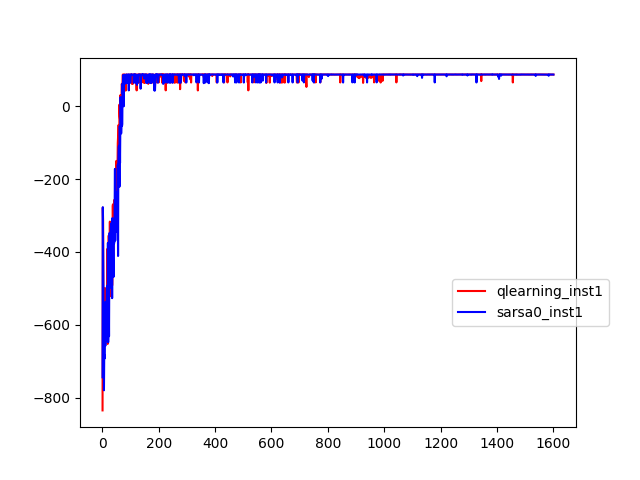
\includegraphics[scale=0.5]{images/qlearn_sarsa0_instance1}
  \caption{Q-learn and Sarsa0 for instance 1}
  \label{fig:ins1}
\end{figure}

\begin{figure}[H]
  \centering
  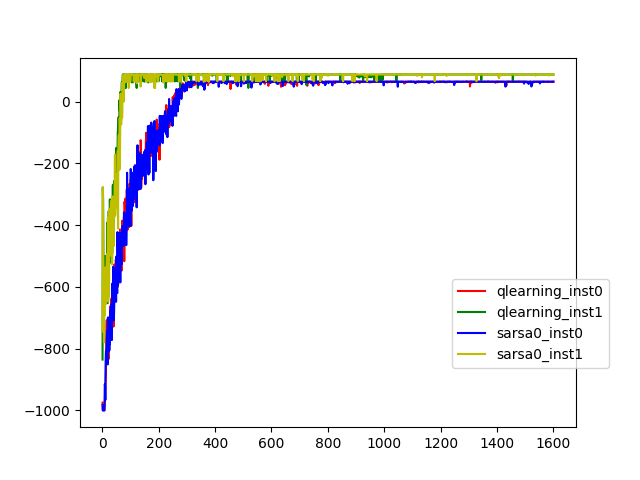
\includegraphics[scale=0.5]{images/qlearn_sarsa0_instance_0_1}
  \caption{Q-learn and Sarsa0 for both instance in the same graph}
  \label{fig:qls0}
\end{figure}

\begin{figure}[H]
  \centering
  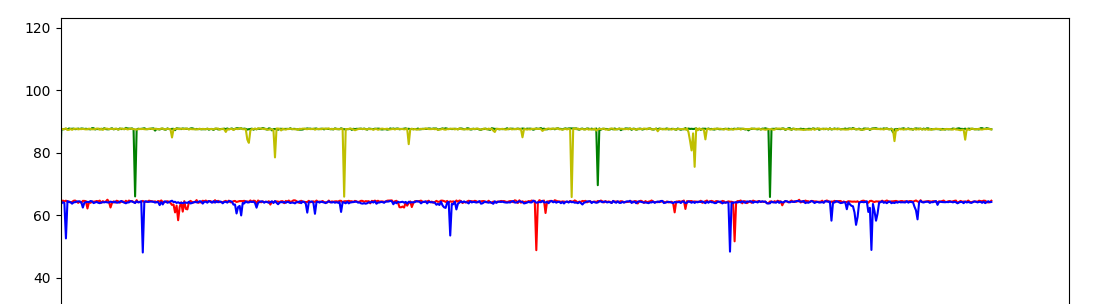
\includegraphics[scale=0.25]{images/close_up_ql_s0_ins0_1}
  \caption{Q-learning and Sarsa0 at optimal value}
  \label{fig:qls0c}
\end{figure}
\end{document}
